\chapter{Uniformity and Stability}
\label{Linearity}
% Uniformity Study 
% New Event recon 
% Linearity Software 

\section{Introduction}
As discussed in chapter \ref{Milan} the experiments demonstrated instability in the uniformity of the detectors (an example of failed detection is seen in figure \ref{fig:UniFail}). We set out to determine the extent of this instability by investigating the uniformity of the detectors. We look to implement protocols to account for detector failure and produce correction maps.
\paragraph{}
The investigations carried out in chapter \ref{Milan} were all performed in \acrshort{HSR}. The work presented here was carried out at \acrlong{UCH} (\acrshort{UCH}) after the system was transported and installed in the nuclear medicine department. Due to the change in environment and transportation the system required a diagnostic test to ensure the system was performing well. The system was found to be functional, however, there were changes of note; the new environment had a high background radiation count than the \acrshort{HSR} lab, and the temperature was also higher, causing the cooling system to be less stable. 

\begin{figure}[!t]
%\vspace{-0.2cm}
\centering
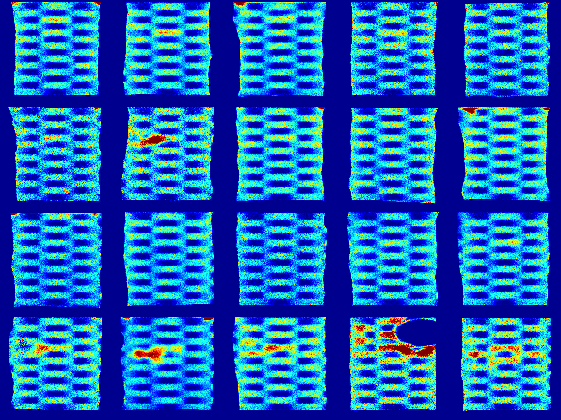
\includegraphics[width=3.6in]{figures/cyl_data.png}

    \caption{The uniformity of each of the 20 detectors shows a number of issues faced, including hot spots and channel failure.} \label{fig:UniFail}
%\vspace{-0.2cm}
\end{figure}

\section{Uniformity}
The experiments at \acrshort{HSR} were time-constrained and so only 2 measures of uniformity were carried out. In this investigation, we mainly included uniformity data from experiments carried out in \acrshort{UCH}. A total of 41 measurements were collected over 6 months on 18 dates. Each uniformity scan required the collimator to be removed, and a point source was placed in the centre of the bore. 

\subsection{Methods}
A measure of uniformity with each detector head was determined through the \acrlong{NEMA} (\acrshort{NEMA}) quality control (QC) procedures for clinical gamma cameras. The \acrshort{NEMA} QC, for a gamma camera which has pixel size $6.4 mm \pm 30\%$, states that a flood scan of 10000 counts in the \acrlong{UFOV} ( \acrshort{UFOV}) or \acrlong{CFOV} (\acrshort{CFOV}) must be carried out. To normalise the uniformity in each acquisition we only consider the first 5 million recorded counts in each detector. We looked at uniformity in the full \acrshort{FOV} and the \acrshort{UFOV} by taking measurements of integral uniformity and the \acrlong{COV} (\acrshort{COV}) for each detector. 
\paragraph{}
Integral uniformity is a measure of global uniformity over the whole planar projection. The maximum and minimum count (C\textsubscript{max} and C\textsubscript{min} respectively) of each detector is calculated. Equation \ref{eqn:IntUni} is used to calculate the integral uniformity as a percentage; the lower the value the greater the uniformity. This, however, is limited by only considering two values from each detector. 

\begin{equation} \label{eqn:IntUni}
        U_{I} = (\frac{C_{max} - C_{min}}{C_{max} + C_{min}})\times100\%
\end{equation}

The \acrshort{COV} is a measure of uniformity which considered all values within a detector. Equation \ref{eqn:CoV} determines the \acrshort{COV} as a percentage of standard deviation (SD) over the mean ($\mu$) of all counts in a given detector. The lower the \acrshort{COV} the greater the uniformity. 

\begin{equation} \label{eqn:CoV}
        CoV = \frac{SD}{\mu}\times100\%
\end{equation}

From the 41 scans, we considered the U\textsubscript{I} and \acrshort{COV} over the whole detector \acrshort{FOV} and \acrshort{UFOV}. The U\textsubscript{I} was used to determine detector failure for each day. As the flood source was located in the centre of all detectors, the system uniformity (figure \ref{fig:systemUI}) was calculated using all counts. Failed detectors were identified by values of  U\textsubscript{system} $> 70\%$. The channel causing the detection failure was identified by anomalous counts (figure \ref{fig:FaultyDay}). After removing the faulty channels we check U\textsubscript{system} (figure \ref{fig:fixsystem} and recalculate the U\textsubscript{I}and \acrshort{COV}. With corrections in place, we can see how the system tends to stability as we learn to implement corrections for detector failure (figure \ref{fig:DailyCOV}). 

\begin{figure}[!t]
%\vspace{-0.2cm}
\centering
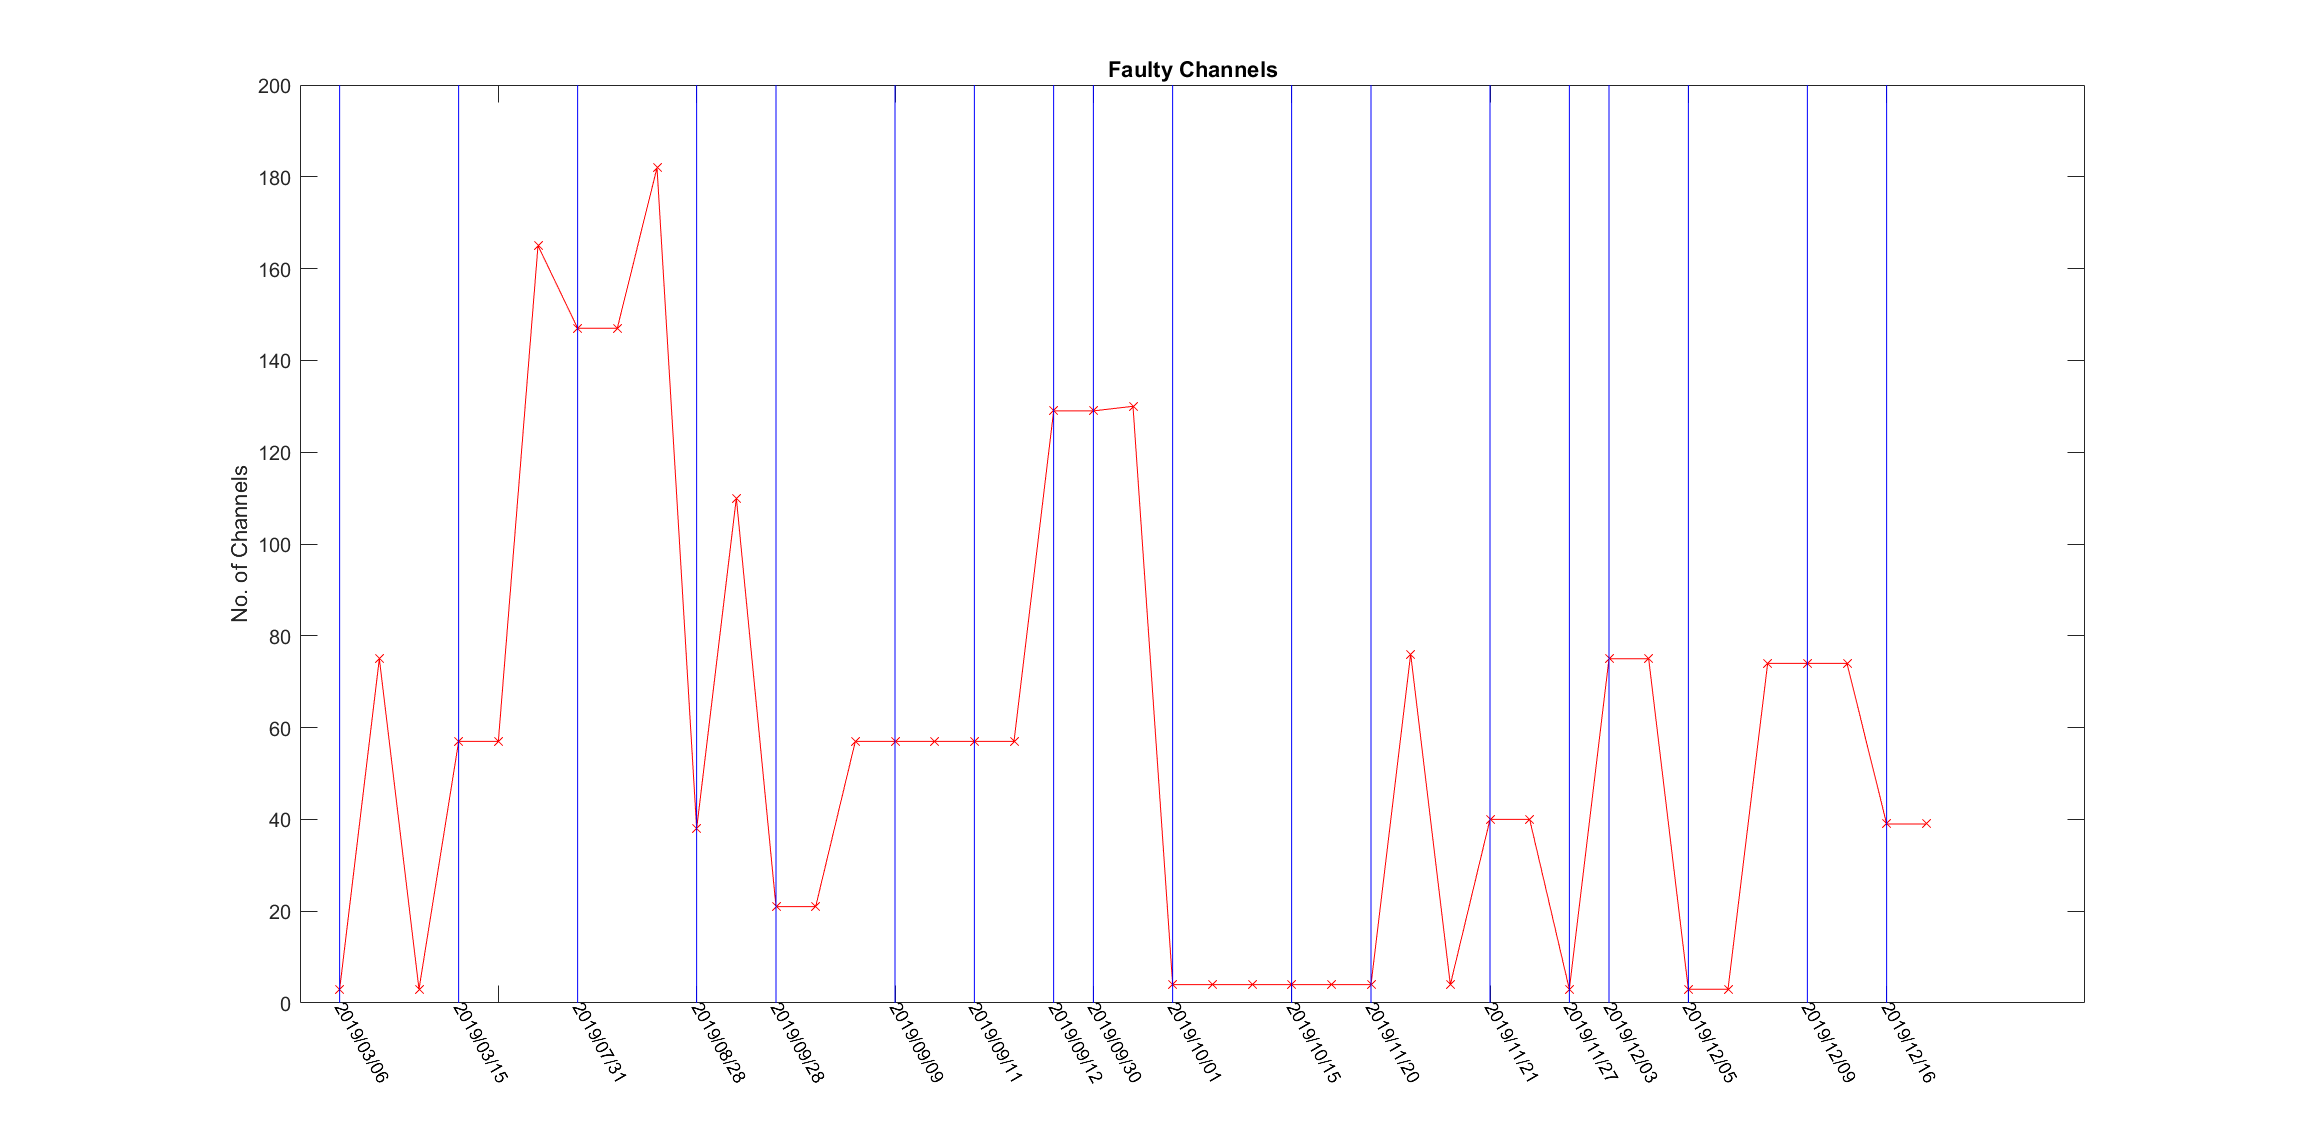
\includegraphics[width=5.5in]{figures/FaultyChannels02.png}

    \caption{The number of faulty channels from each day of the study. Large corrections was carried out to fix channels on several occasions.} \label{fig:FaultyDay}
%\vspace{-0.2cm}
\end{figure}

\begin{figure}[!tbp]
  \centering
  \subfloat[System uniformity with failed channels present. This gives very poor uniformity due to hot spots and dead pixels. ]{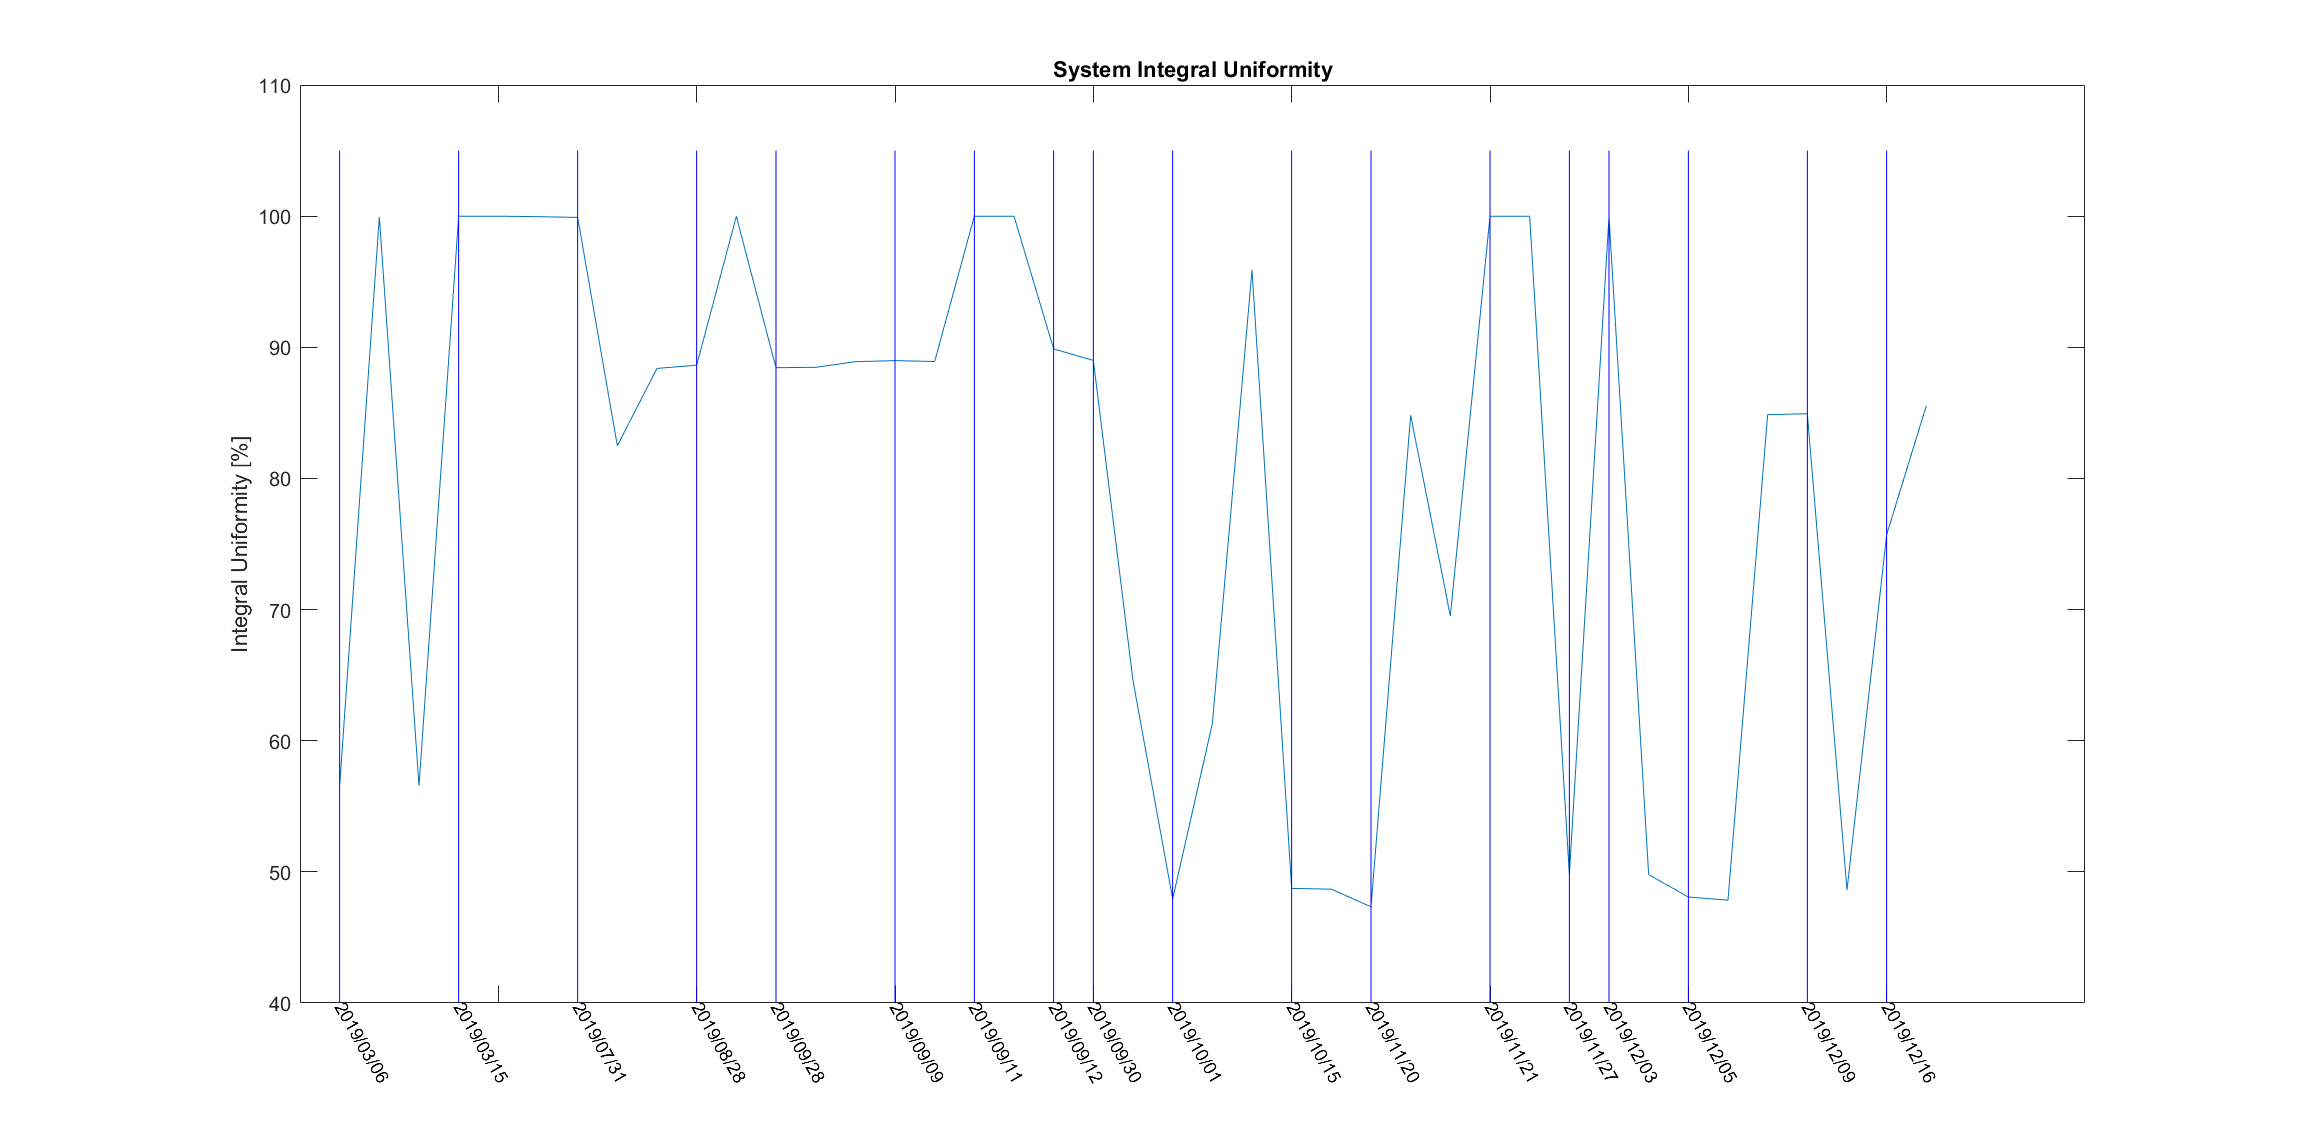
\includegraphics[width=1.1\textwidth]{figures/IUSystem_PreFix.png}\label{fig:systemUI}}
  \hfill
  \subfloat[Correcting for channel failure gives a greater uniformity across the whole system.]{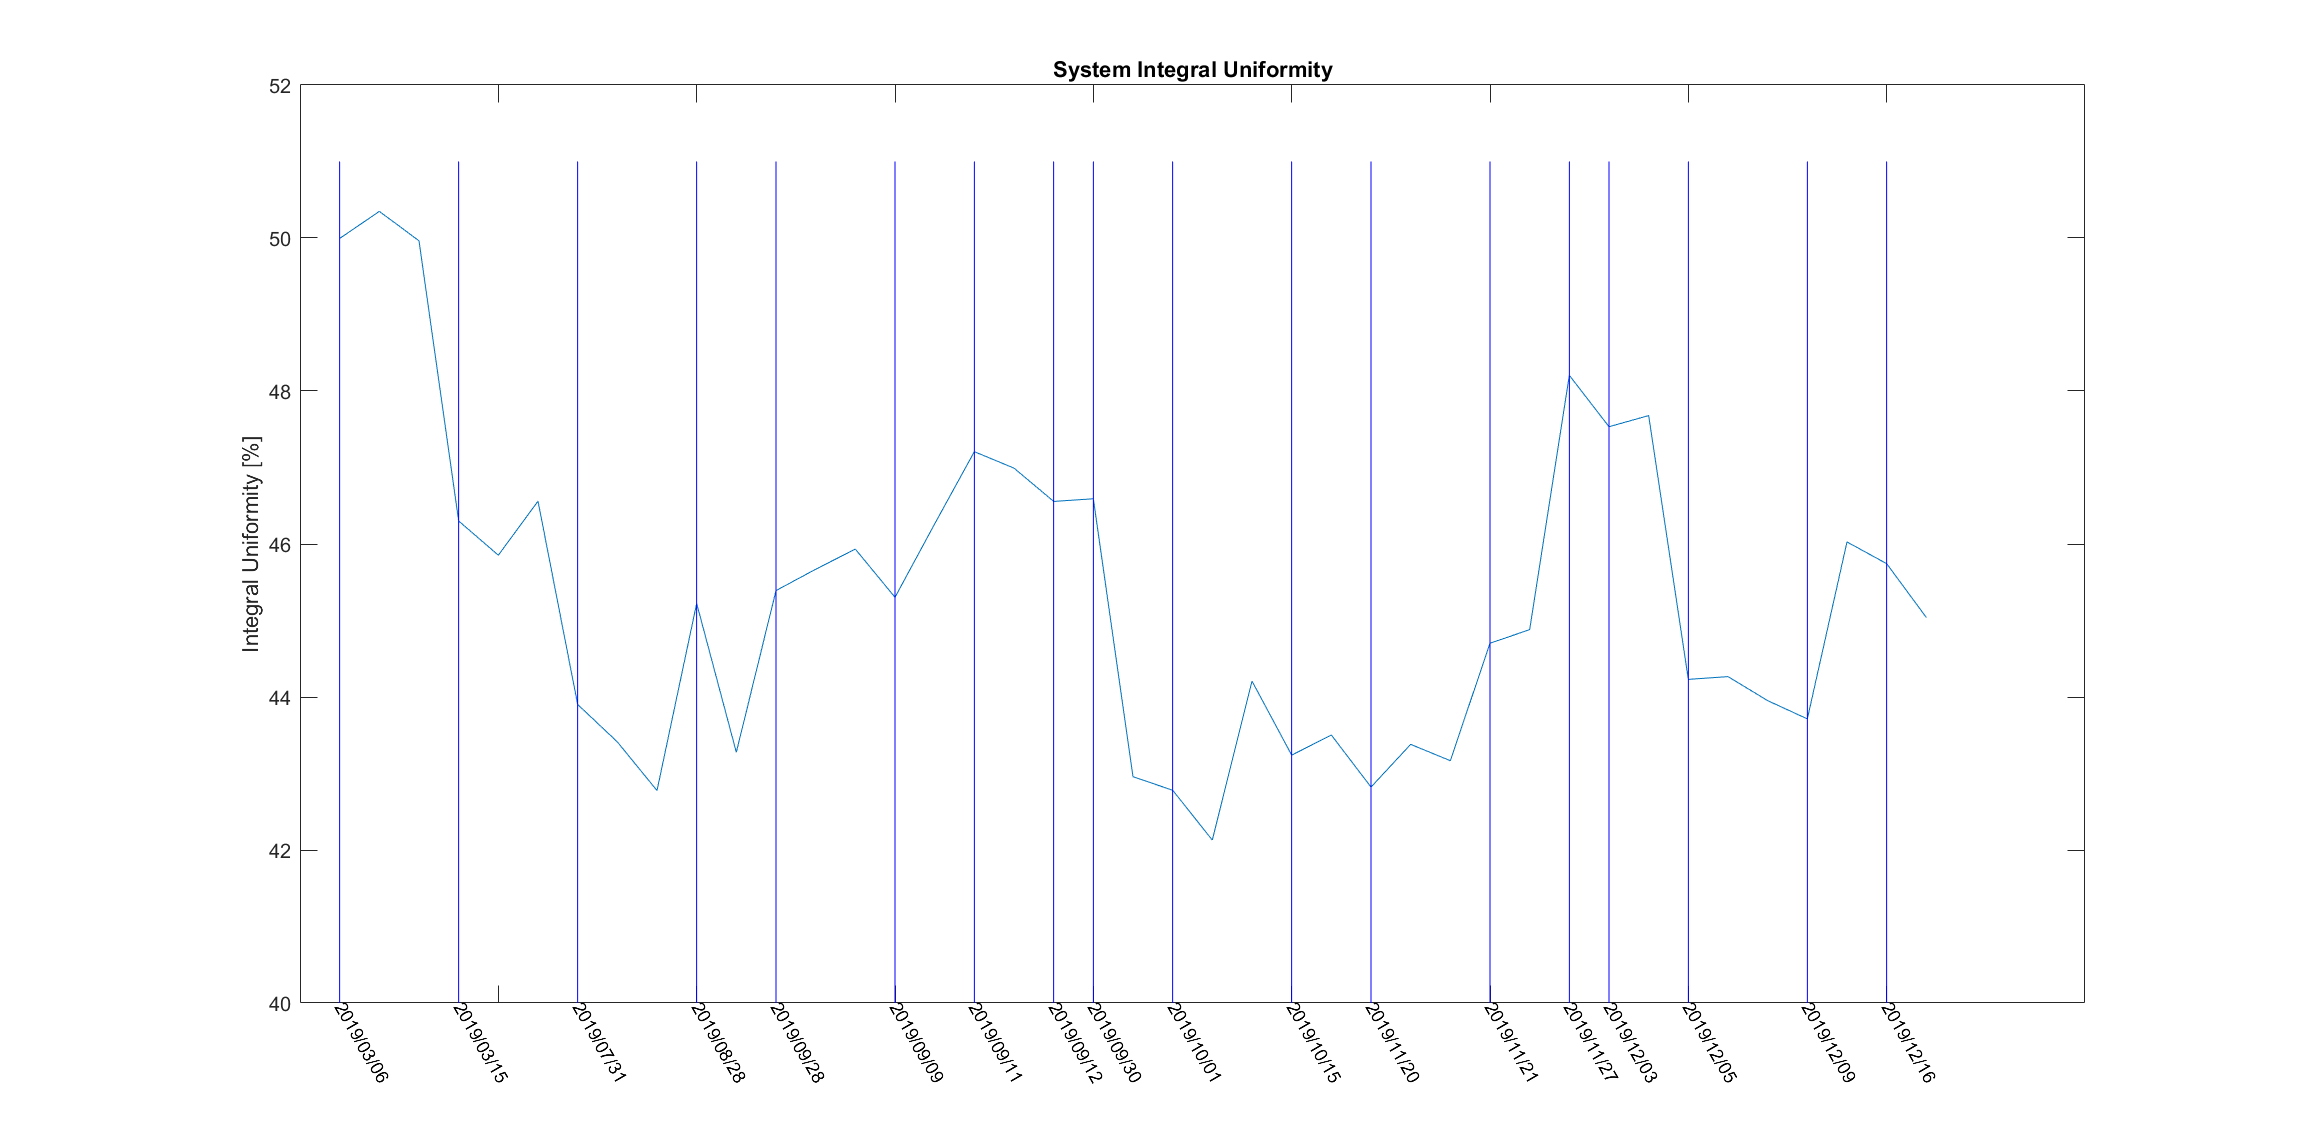
\includegraphics[width=1.1\textwidth]{figures/IUSystem.png}\label{fig:fixsystem}}
  \caption{This measure is used to determine an overall uniformity of the system however we must consider the detector heads separately for an accurate measure of uniformity.}
\end{figure}

\begin{figure}[!t]
%\vspace{-0.2cm}
\centering
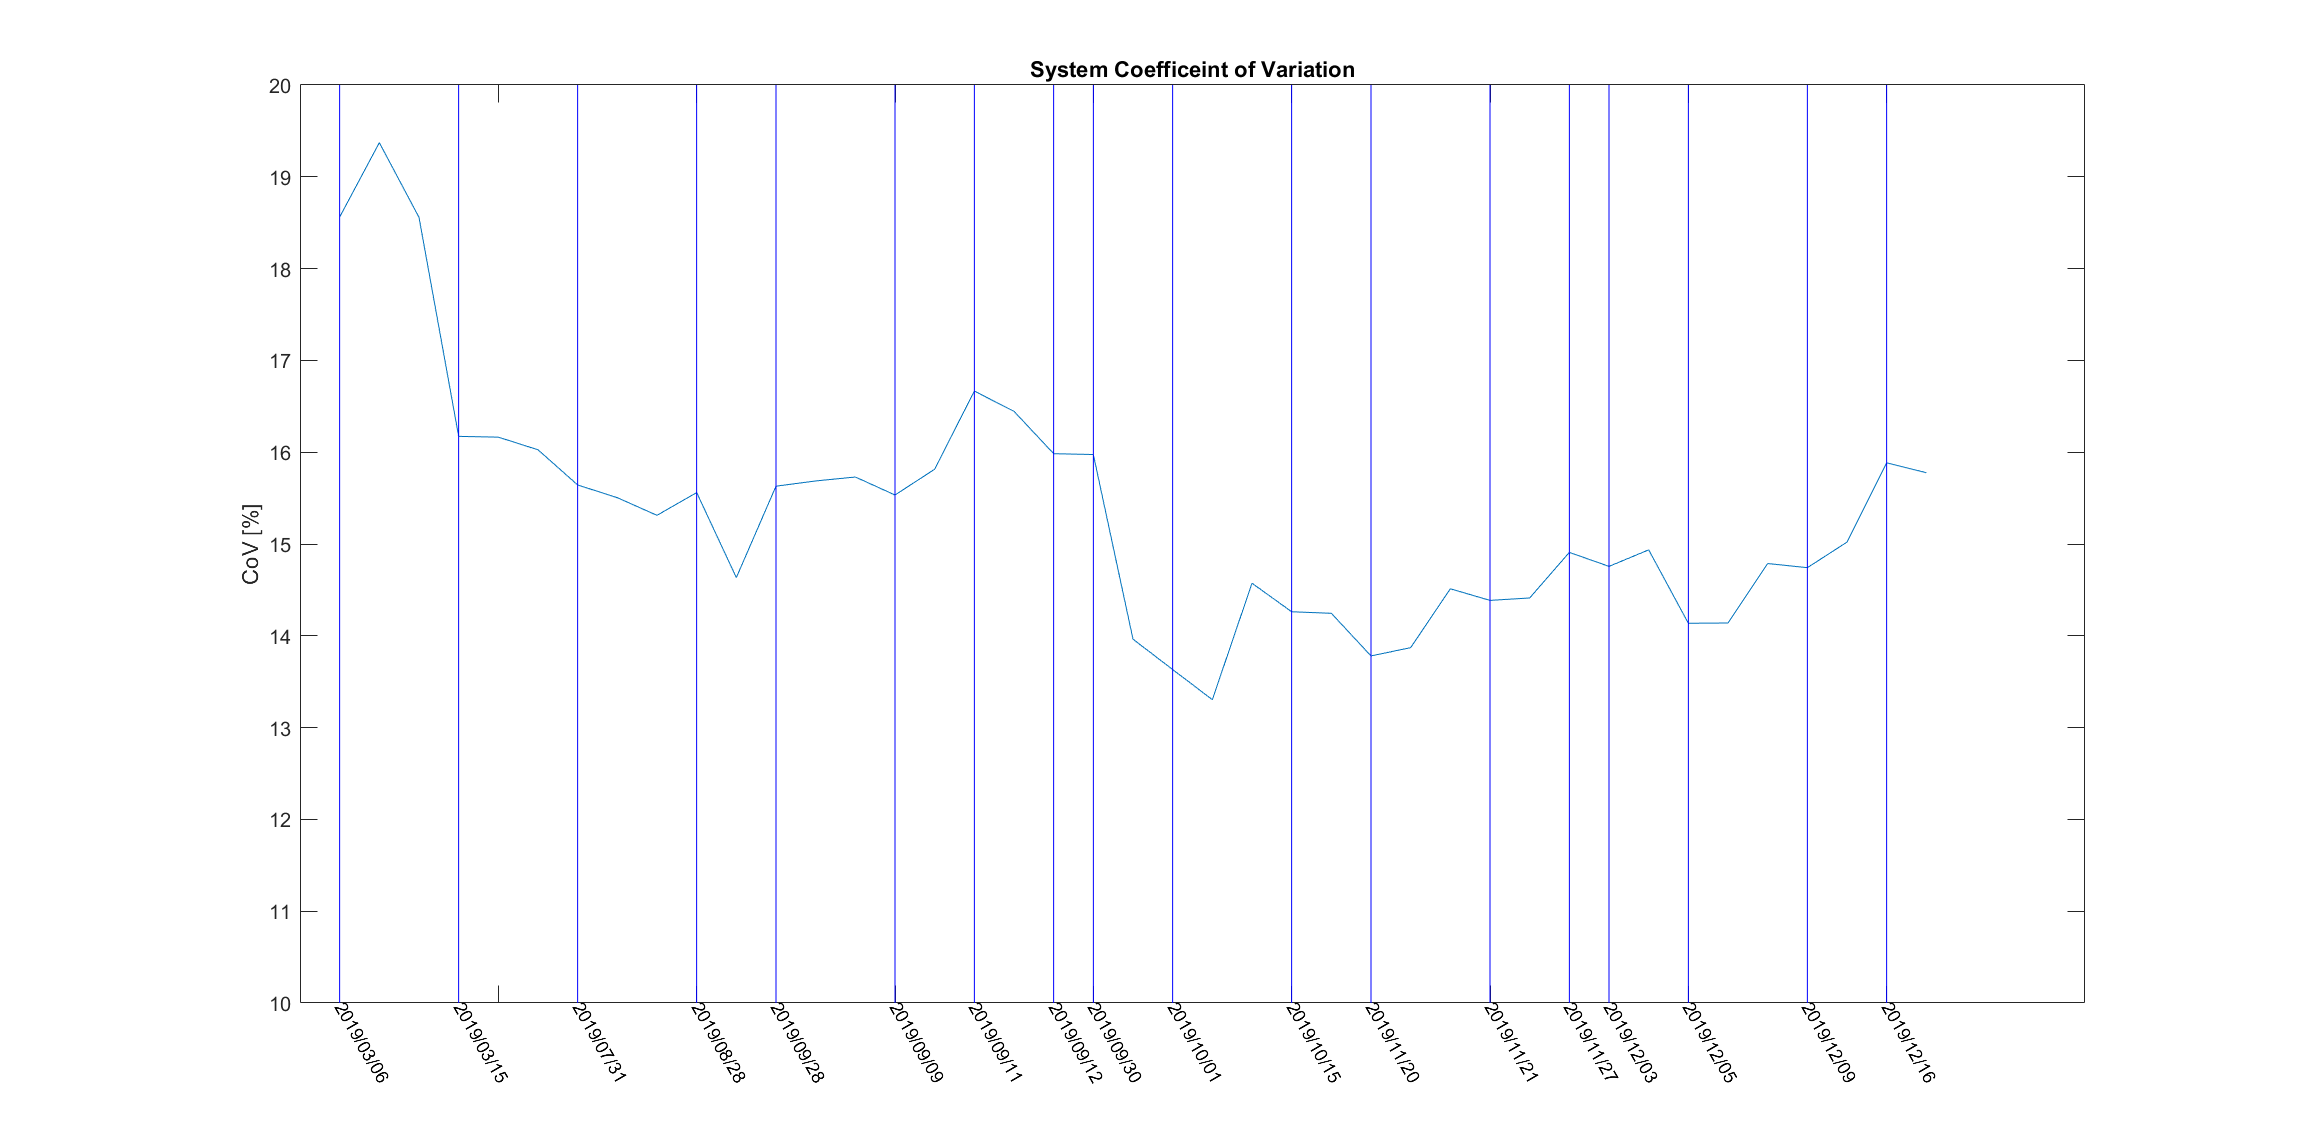
\includegraphics[width=5.5in]{figures/COVSystem.png}

    \caption{The \acrshort{COV} is measured for each day of the study. This shows variation within daily measures but also key dates which corrections were applied.} \label{fig:DailyCOV}
%\vspace{-0.2cm}
\end{figure}


\subsection{Results}
We first consider raw uniformity data. Figures \ref{fig:RawUBox} and \ref{fig:RawCovBox} show box plots of the uniformity study. Faulty detectors are immediately identified by the high variation and poor uniformity. The \acrshort{UFOV} improves the uniformity slightly as the edge of the detectors have greater distortion and are not considered in reconstruction. However, the stability of the channels is independent of the \acrshort{FOV} and so figures \ref{fig:UFOVUBox} and \ref{fig:UFOVCovBox} shows little improvement in detector uniformity. We must consider healthy channels to gauge uniformity of the detectors.

\begin{figure}[!t]
%\vspace{-0.2cm}
\centering
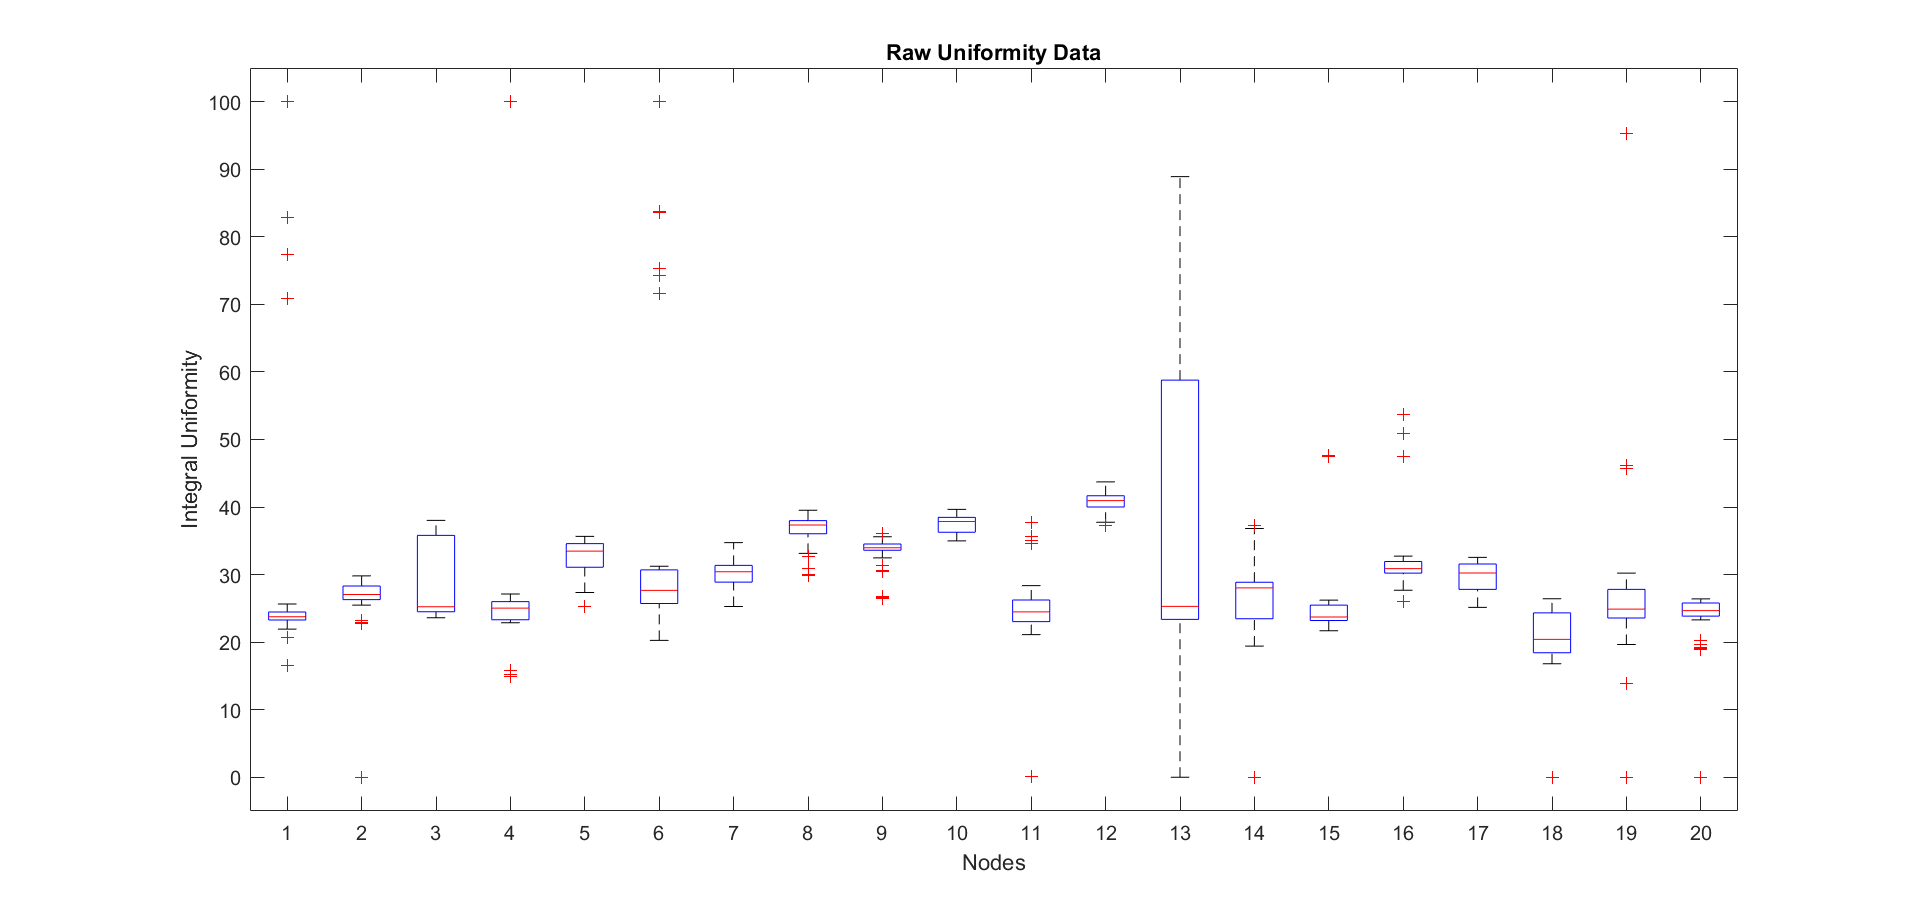
\includegraphics[width=5.6in]{figures/RawUBox.png}

    \caption{The integral uniformity of each detector demonstrates instability in detectors with large number of faulty channels. This plot does not show consistent channel failure within detector 16 for example, which requires correction but is consistent in its failure. Large values show days with anomalous channel failure. } \label{fig:RawUBox}
%\vspace{-0.2cm}
\end{figure}

\begin{figure}[!t]
%\vspace{-0.2cm}
\centering
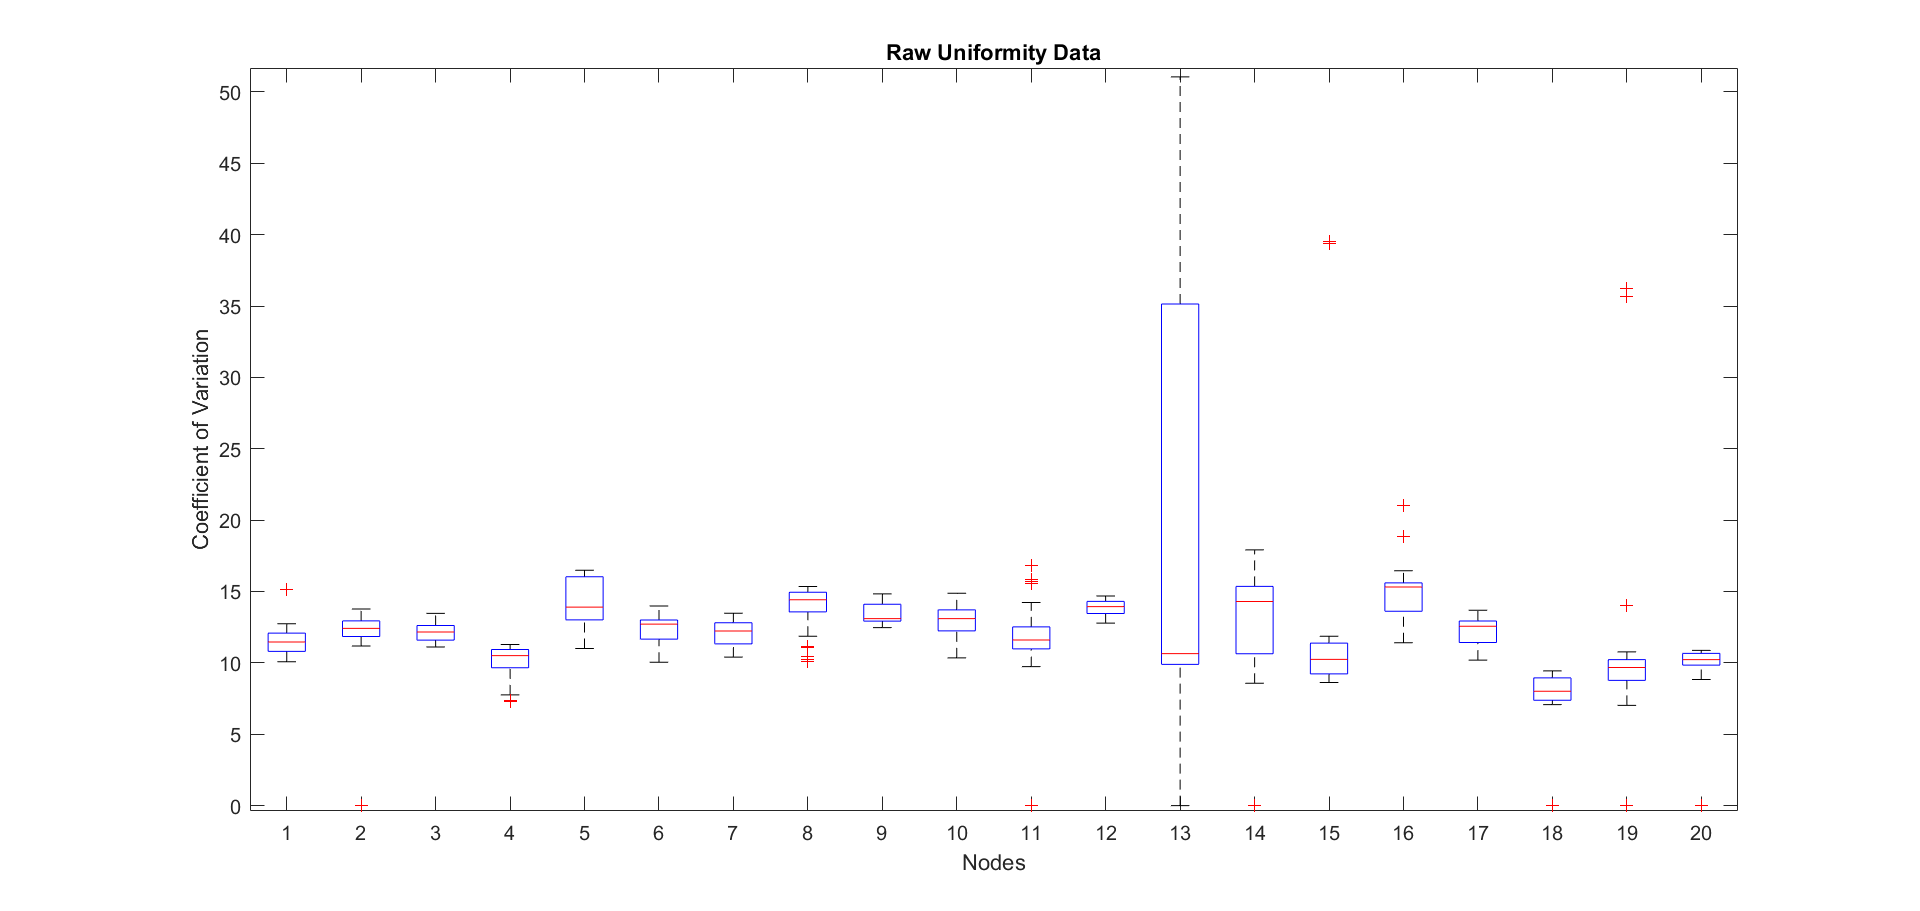
\includegraphics[width=5.6in]{figures/RawCOVBox.png}

    \caption{The \acrshort{COV} of each detector gives an indication of uniformity between channels. Before correction we cannot distinguish channel failure from non-uniformity.} \label{fig:RawCovBox}
%\vspace{-0.2cm}
\end{figure}

\begin{figure}[!t]
%\vspace{-0.2cm}
\centering
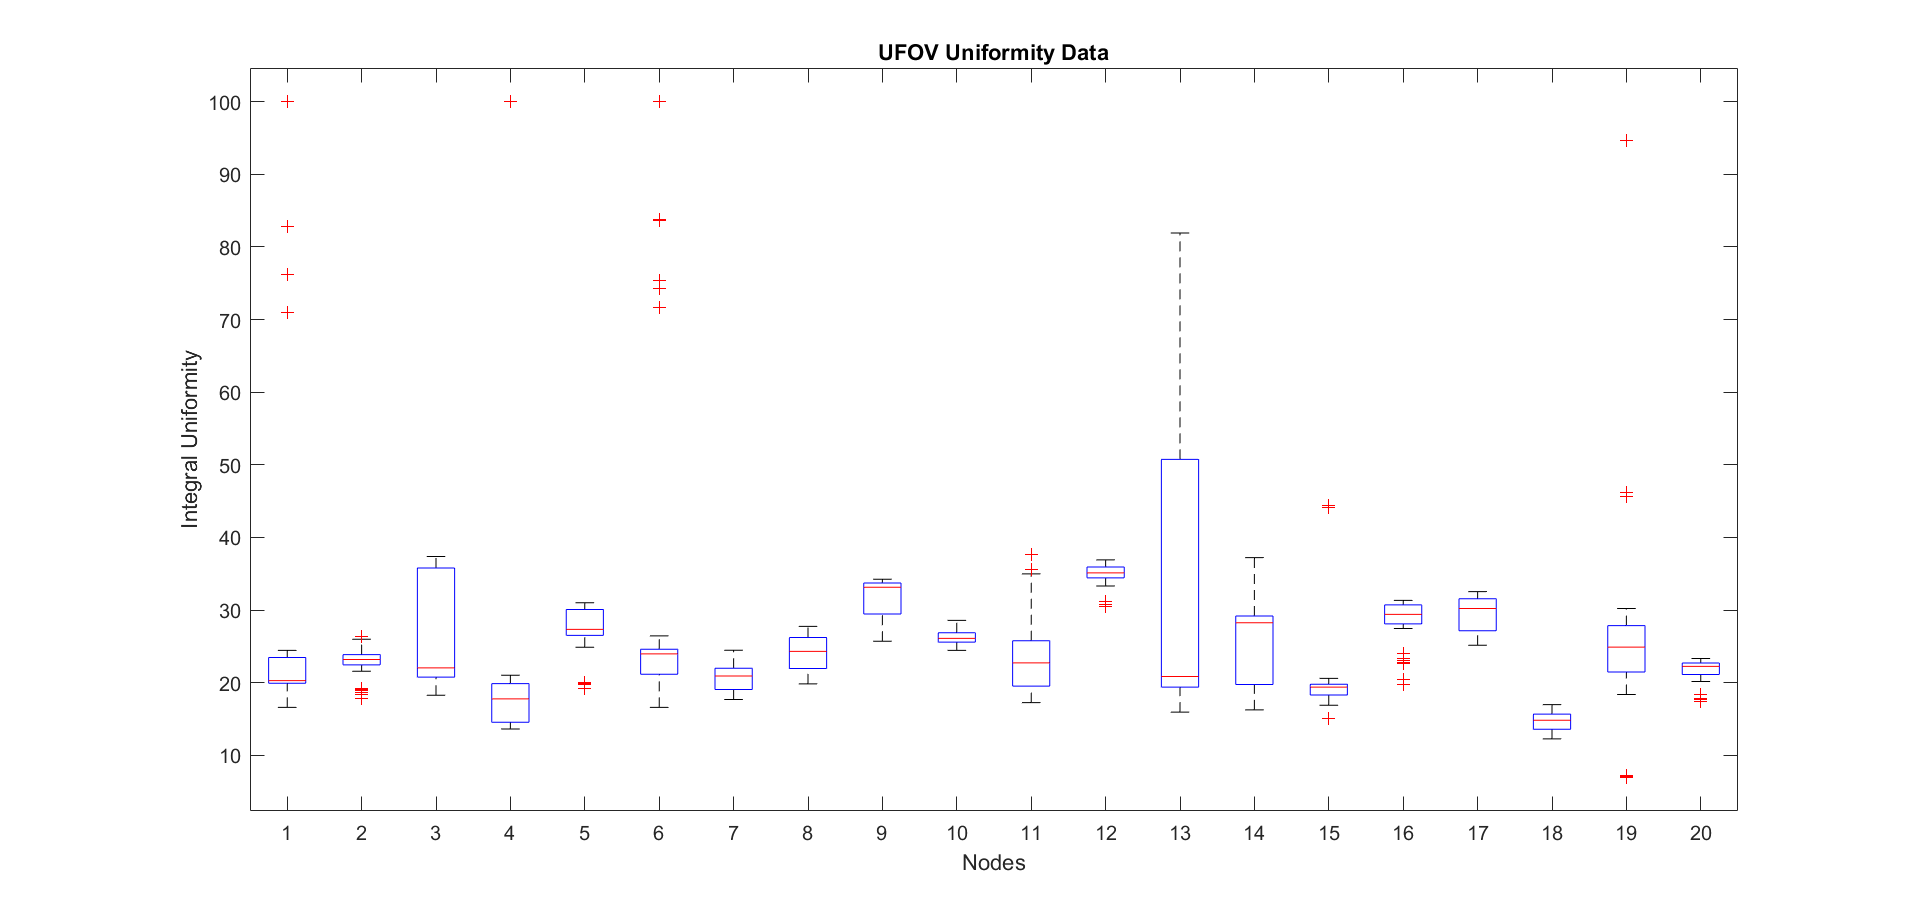
\includegraphics[width=5.6in]{figures/UFOVUBox.png}

    \caption{Considering the \acrshort{UFOV} will improve linearity but is independent of uniformity and stability in the presence of faulty channels.} \label{fig:UFOVUBox}
%\vspace{-0.2cm}
\end{figure}

\begin{figure}[!t]
%\vspace{-0.2cm}
\centering
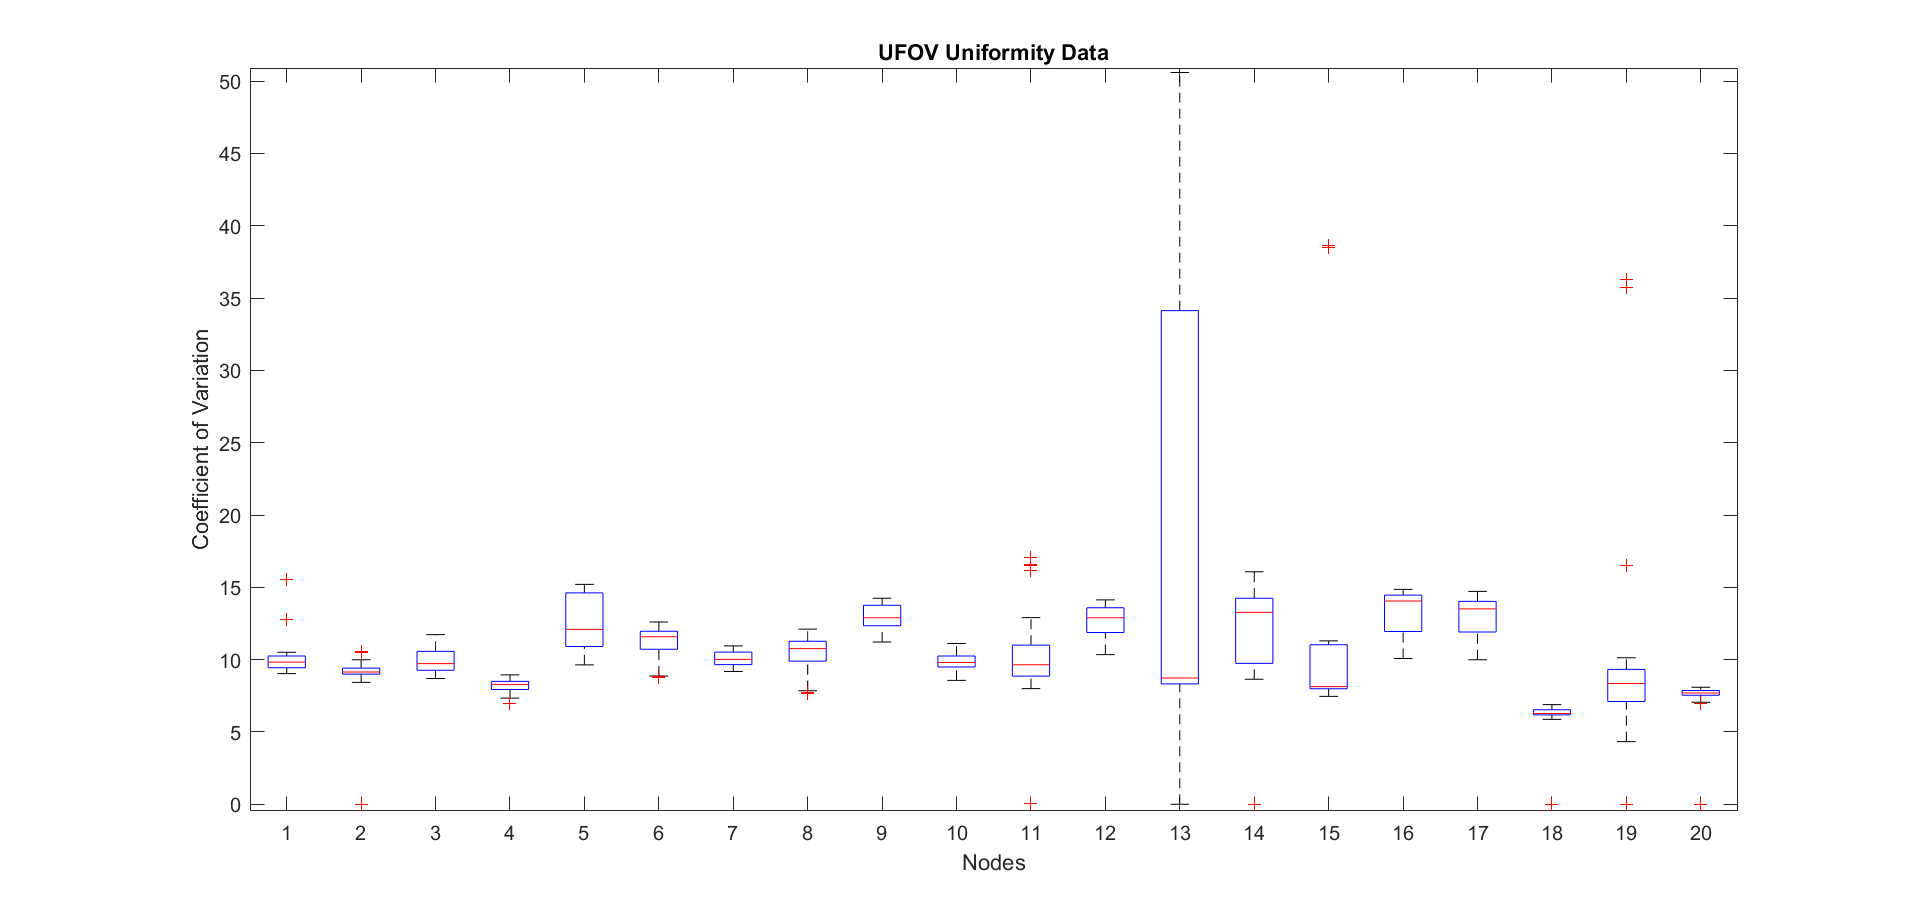
\includegraphics[width=5.6in]{figures/UFOVCOVBox.png}

    \caption{Great instability in the channels drowns out any meaningful distinction within the \acrshort{COV}.} \label{fig:UFOVCovBox}
%\vspace{-0.2cm}
\end{figure}

Figure \ref{fig:HealthUI} shows U\textsubscript{I} for the healthy channels. The presence of a faulty channel did not define poor uniformity as many detectors with few faults have lower U\textsubscript{I} than those with many faults. However, detectors, such as 13, which had faults for large periods gave a wide spread of values. Detectors with consistently poor uniformity suggest the presence of undetected faults. 
The integral uniformity is not an effective measure for detectors with faults and high variability as it only considers the extreme values. We consider the \acrshort{COV} for the healthy channels (figure \ref{fig:HealthCOV}). This has a smaller spread due to detector failure as shown in detector 13, suggesting the remaining healthy channels are more uniform. However faulty detectors have fewer channels so will present less variation. 

\begin{figure}[!t]
%\vspace{-0.2cm}
\centering
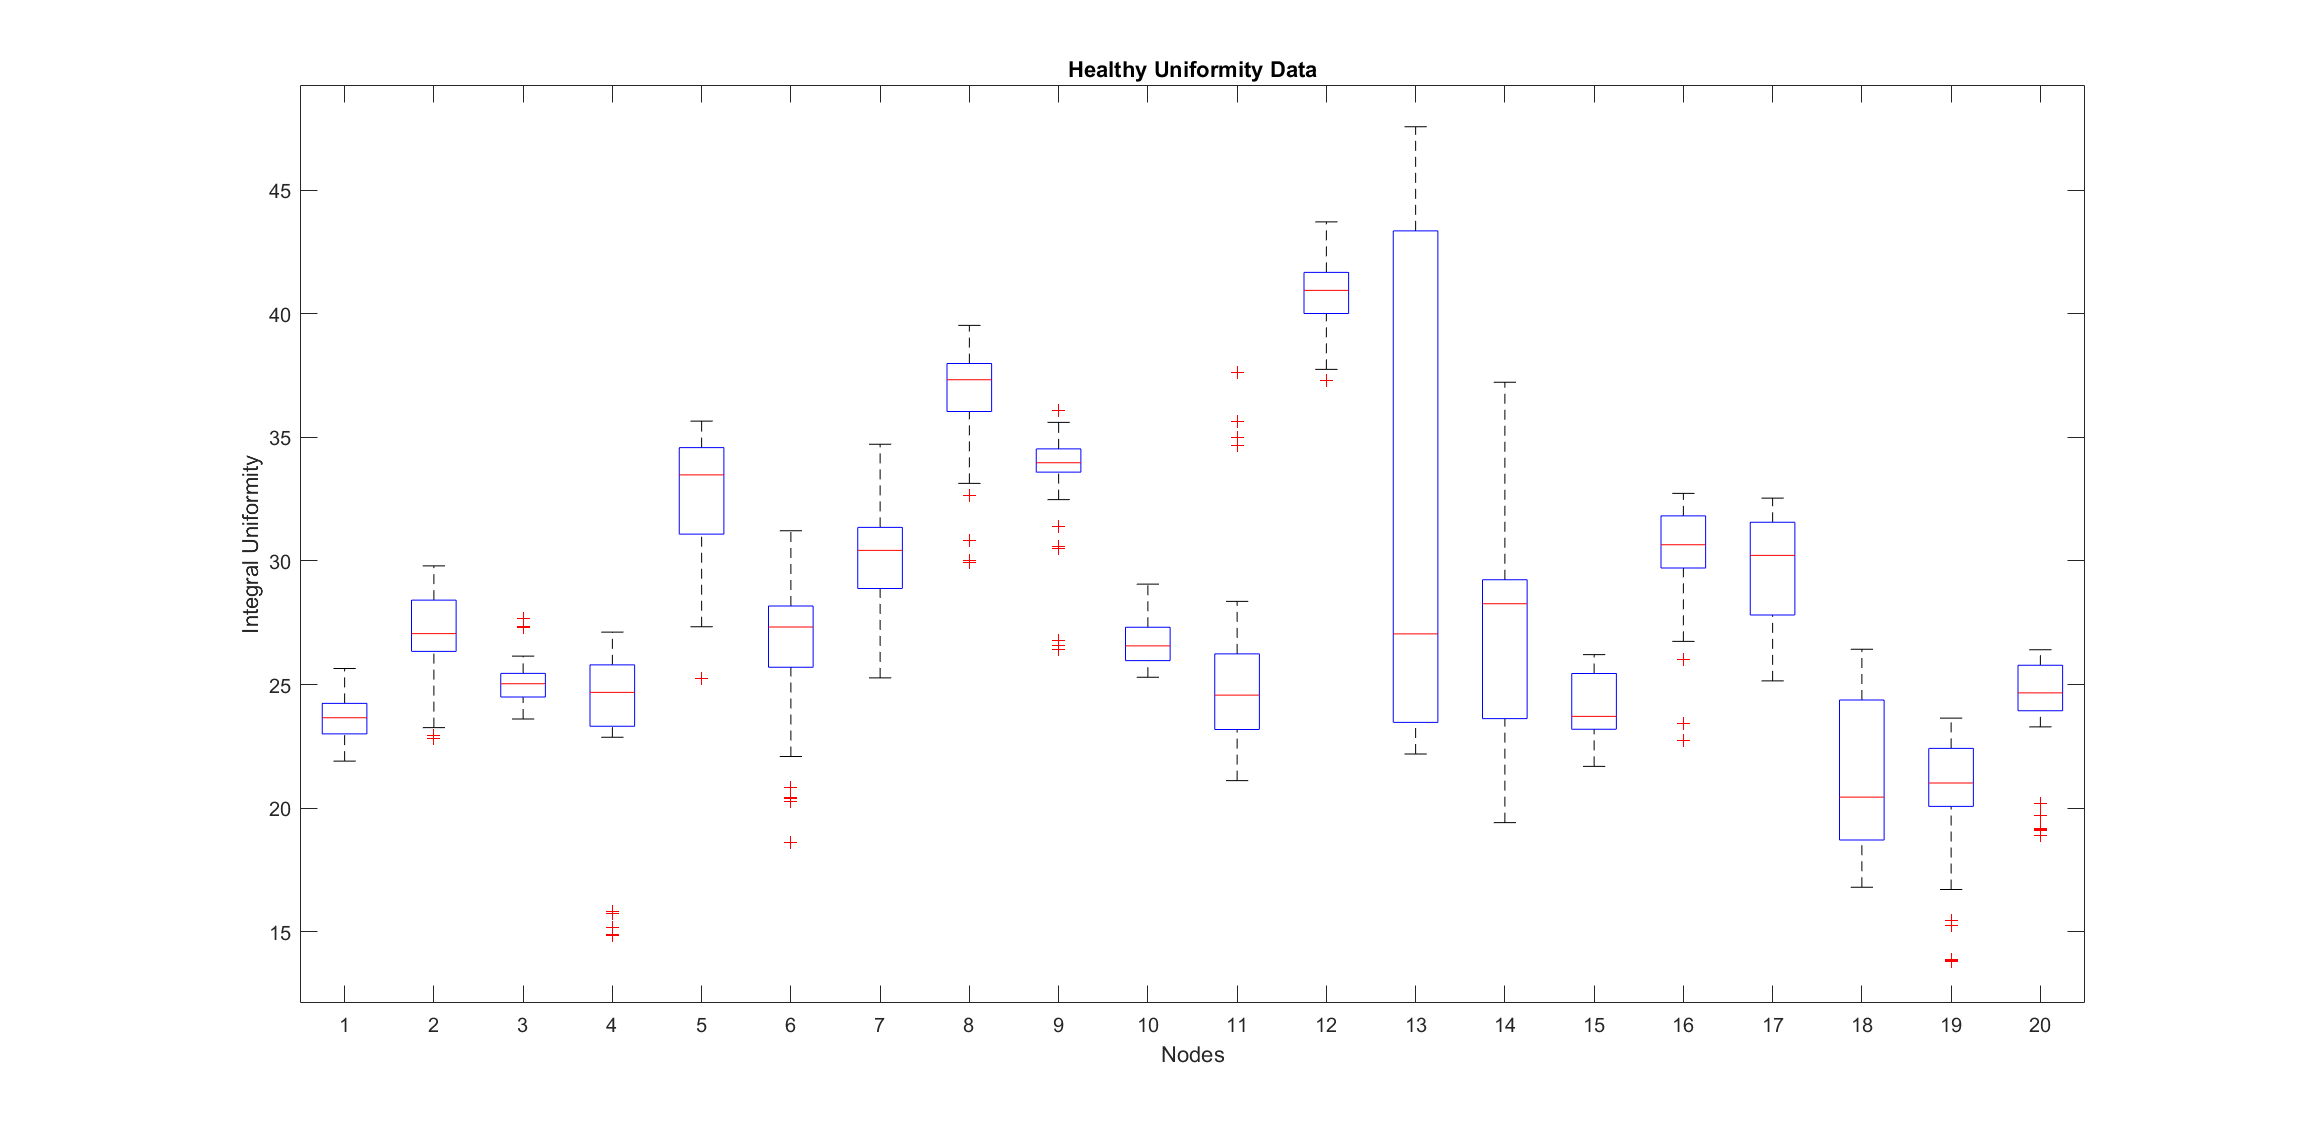
\includegraphics[width=5.6in]{figures/FixUBox.png}

    \caption{The removal of faulty channels shows are more reliable measure of uniformity. These plots now show the variation in uniformity due to detector instability and not due to failed pixels.} \label{fig:HealthUI}
%\vspace{-0.2cm}
\end{figure}

\begin{figure}[!t]
%\vspace{-0.2cm}
\centering
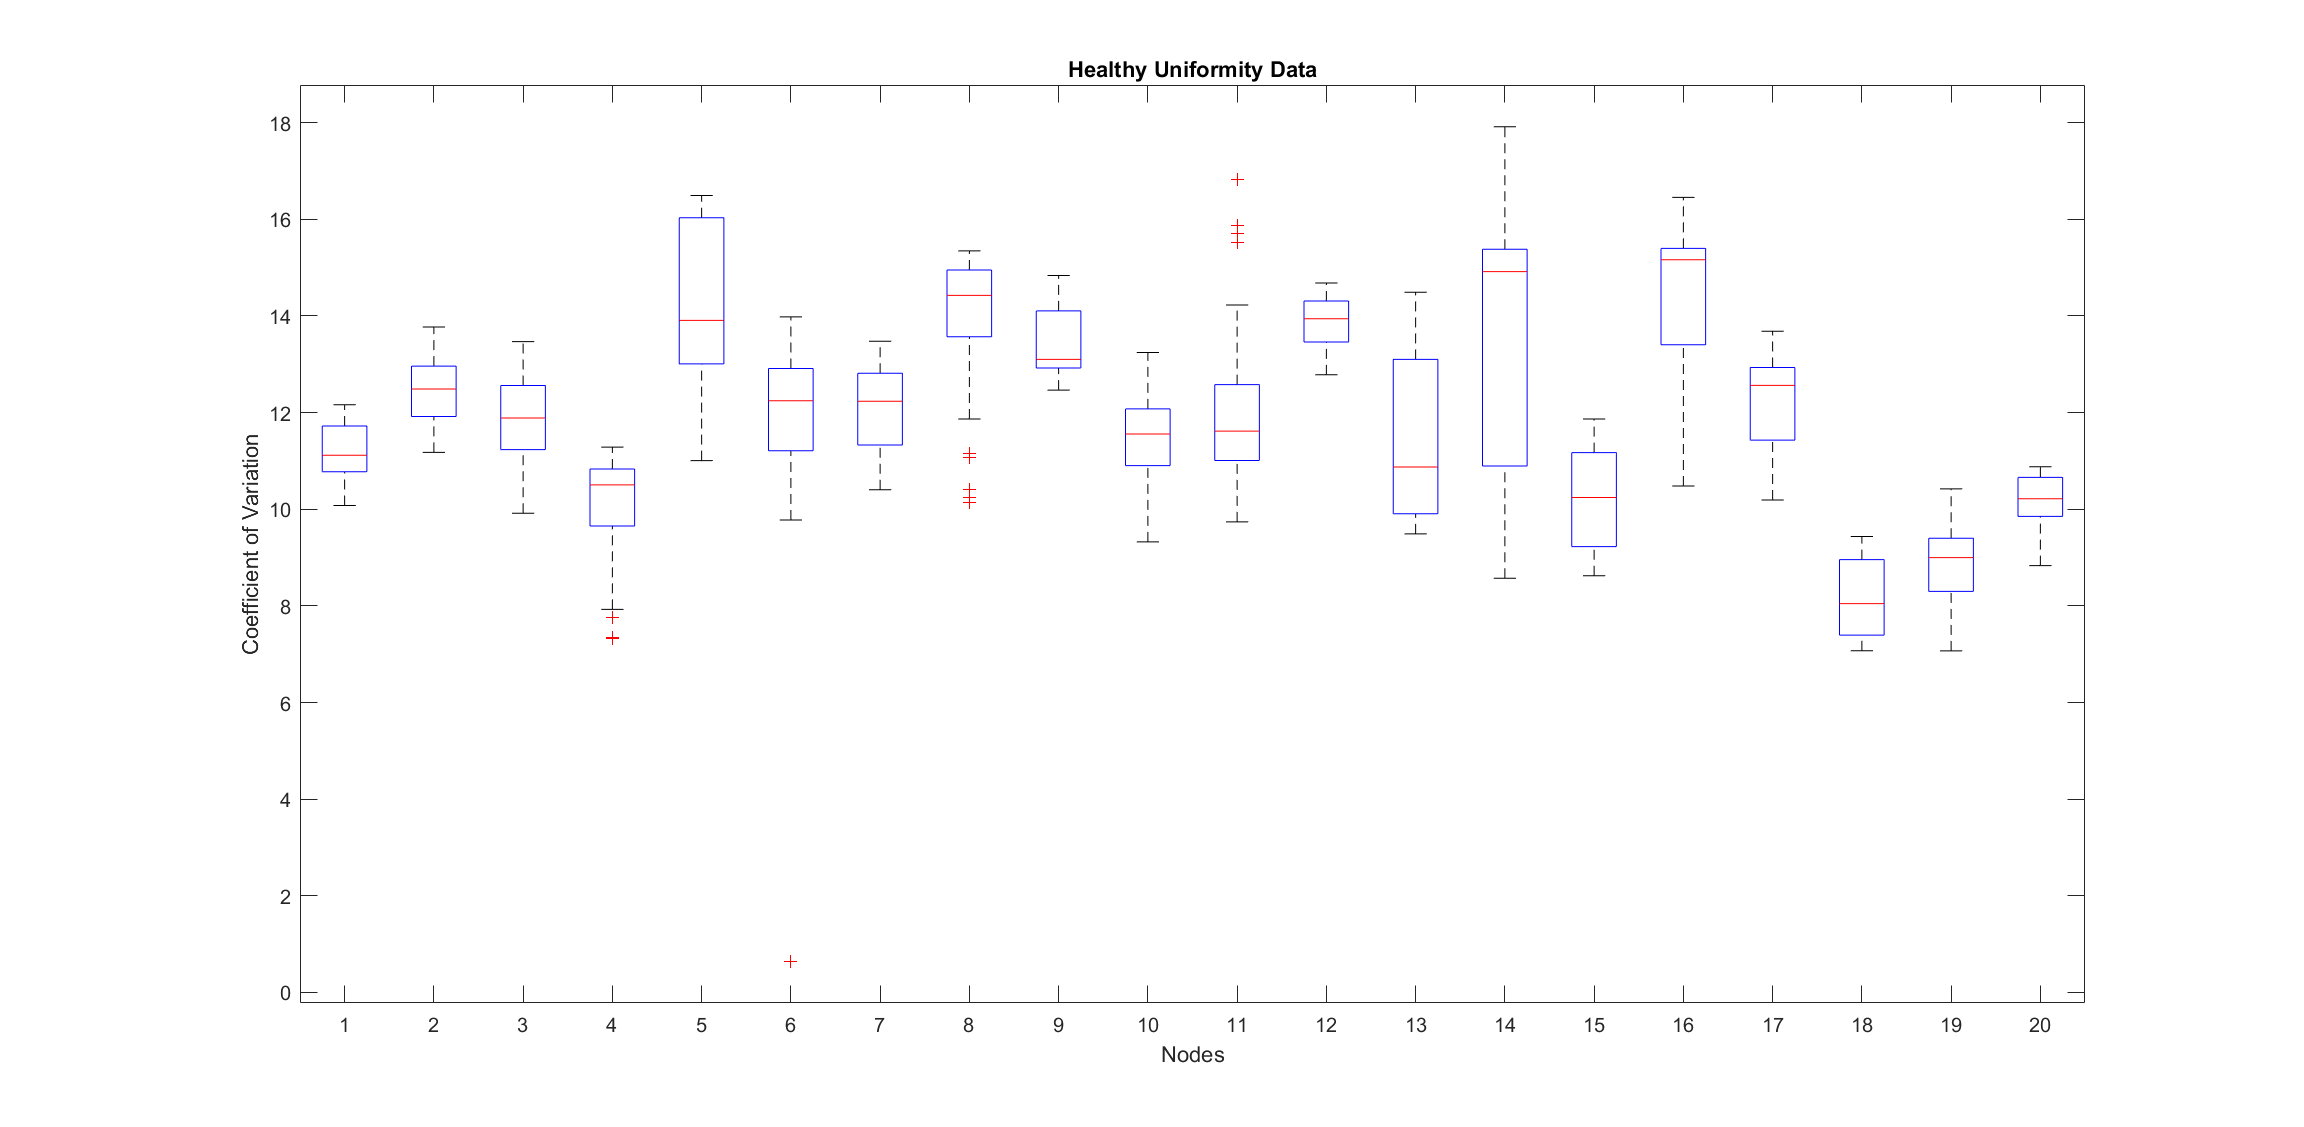
\includegraphics[width=5.6in]{figures/FixCOVBox.png}

    \caption{The \acrshort{COV} is independent of the failed channels as shown in detector 13 which has a more consistent \acrshort{COV} when failed channels are removed.} \label{fig:HealthCOV}
%\vspace{-0.2cm}
\end{figure}

Finally, the \acrshort{UFOV} was considered over the healthy channels. From figure \ref{fig:healthUFOVU} and \ref{fig:healthUFOVCOV} it is clear that the unstable channels can still demonstrate a good uniformity once the corrections are applied. The uniformity between detectors are independent as they act as separate units, however, they share a geometric relation. As stated, the scanning room had a high background count which was subject to the position of the scanner; if one side of the detectors is closer to a source then it stands to reason that these detectors will share similar non-uniformity due to the source proximity. 

\begin{figure}[!t]
%\vspace{-0.2cm}
\centering
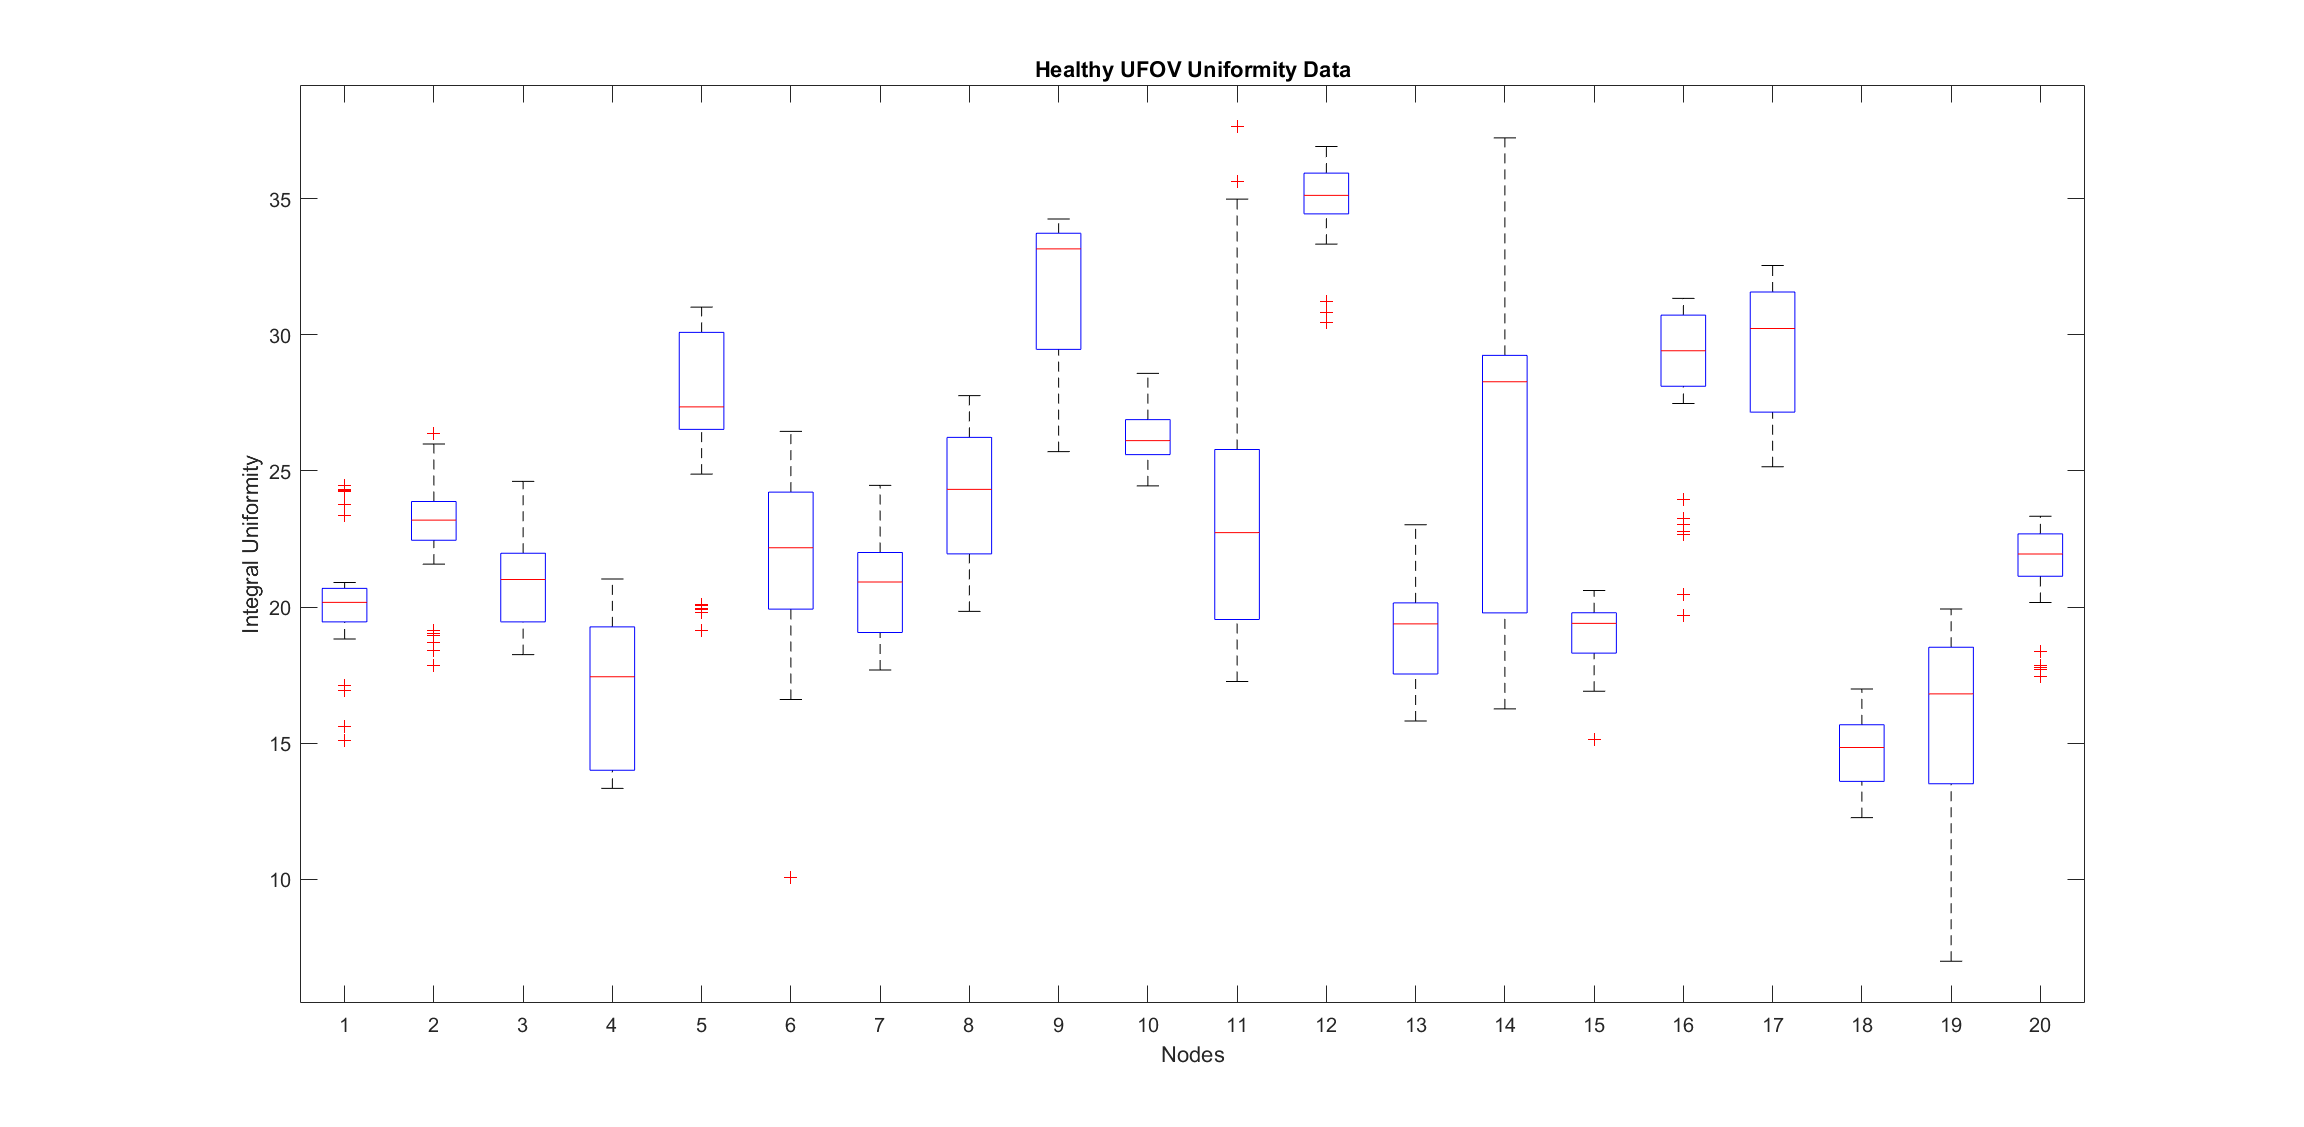
\includegraphics[width=5.6in]{figures/FixUFOVUBox.png}

    \caption{With the \acrshort{UFOV} and channel corrections we can now determine the detector uniformity and stability. This shows a greater stability and uniformity within the individual detectors.} \label{fig:healthUFOVU}
%\vspace{-0.2cm}
\end{figure}

\begin{figure}[!t]
%\vspace{-0.2cm}
\centering
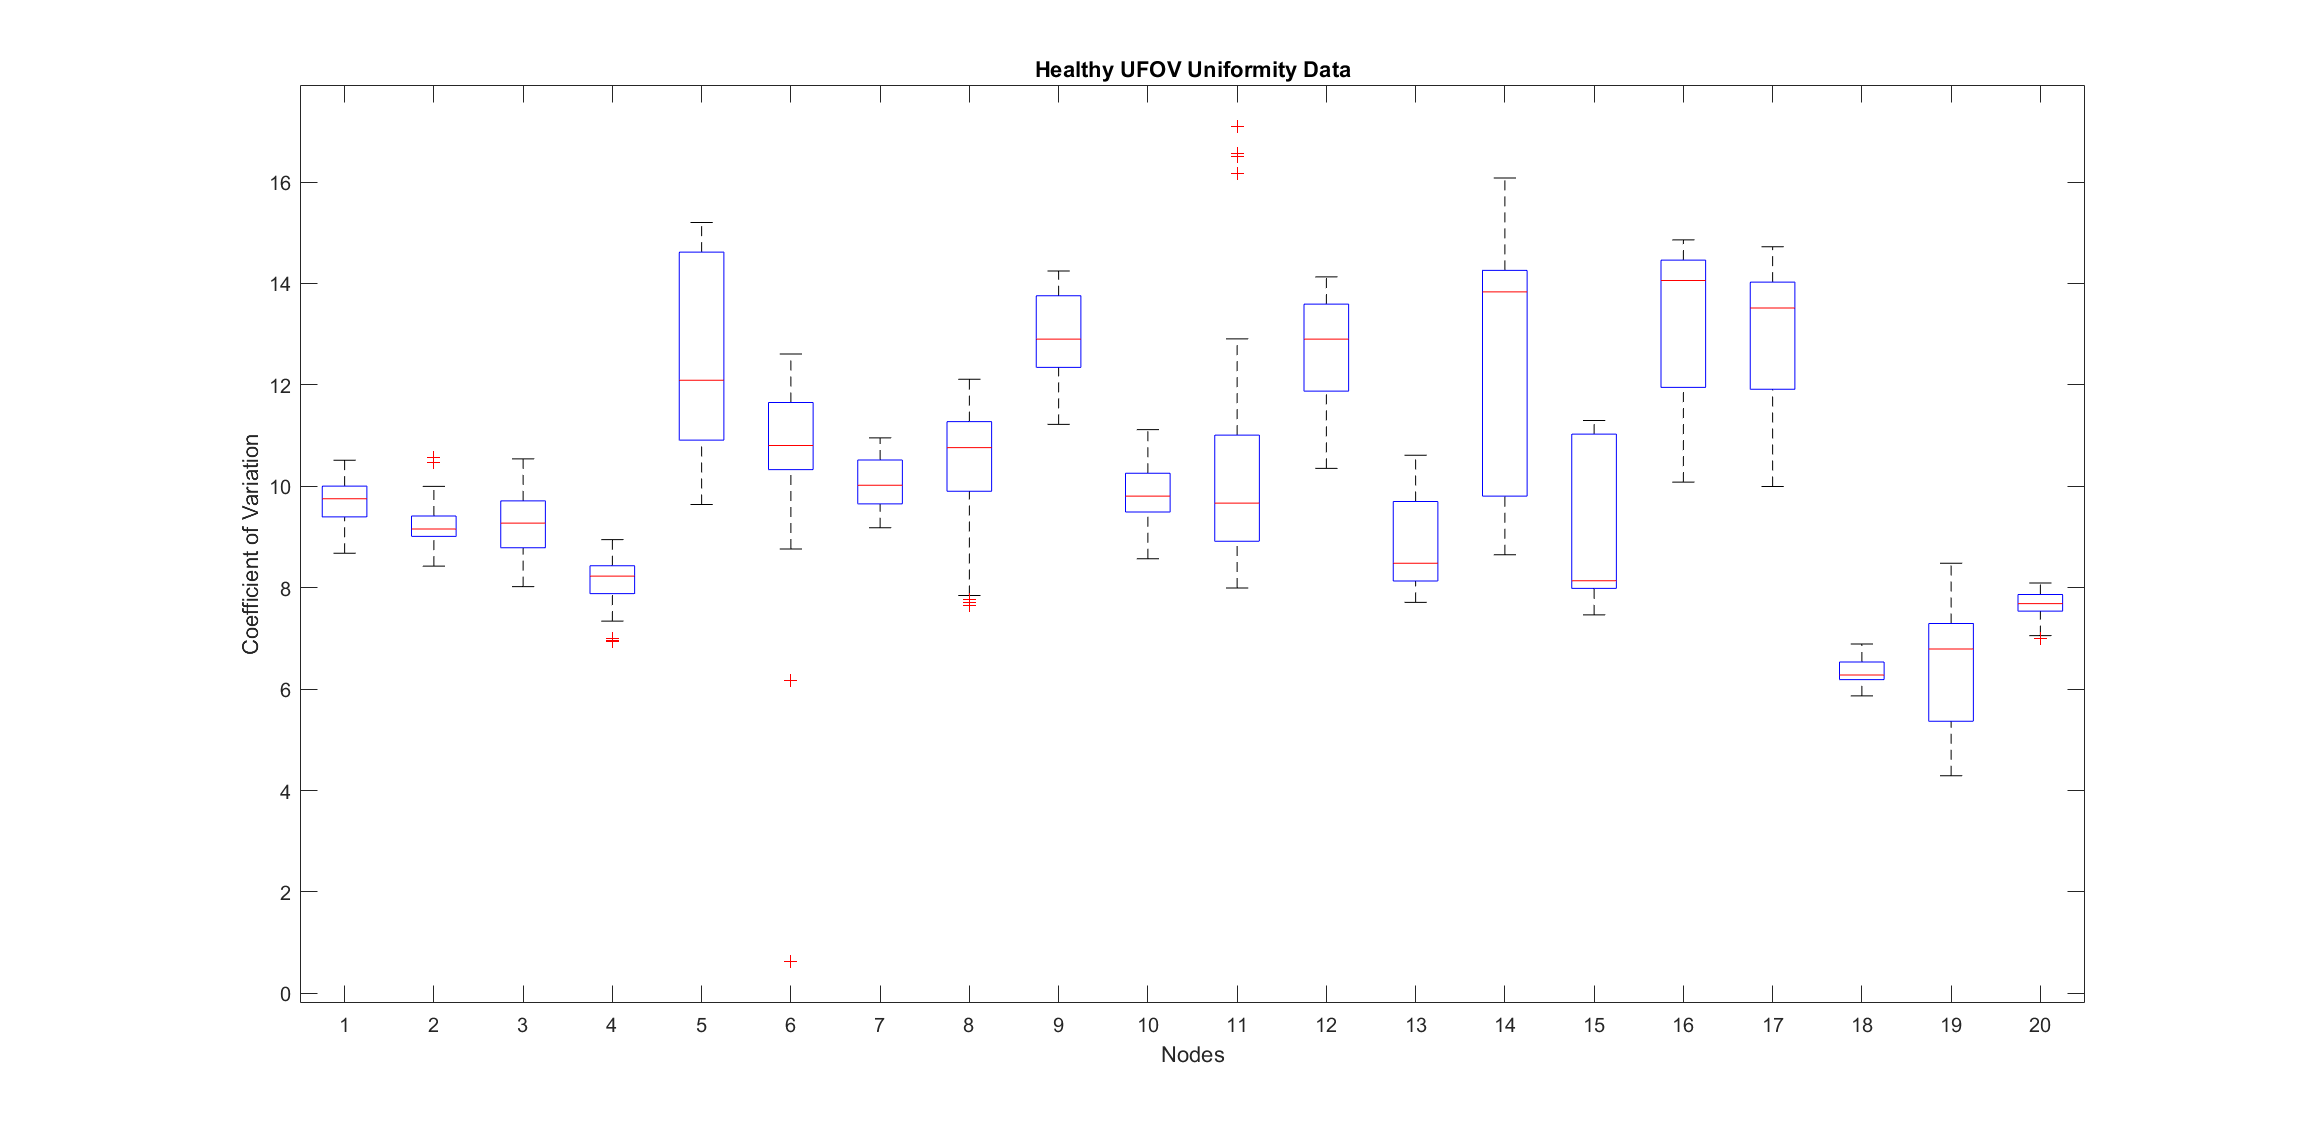
\includegraphics[width=5.6in]{figures/FixUFOVCOVBox.png}

    \caption{The difference in \acrshort{COV} between detectors suggests further investigation is required. We must determine why some detectors appear to be healthier than others.} \label{fig:healthUFOVCOV}
%\vspace{-0.2cm}
\end{figure}

\subsection{Discussion}
The integral uniformity gave a good measure to identify faulty channels and determine the need for manual intervention. We look to establish a standard baseline in which to measure future uniformity. With more scans, we can determine a suitable value of U\textsubscript{I} which will give an acceptable level of detector uniformity. The \acrshort{COV} values over all scans give a measure of detector stability. The \acrshort{COV} of a given detector over the 41 scans revealed how stable the uniformity was within the 6 months. We can use this to diagnose the health of the detector and make decisions replacement or fixes. 
\paragraph{}
Figure \ref{fig:FaultyDay} reveals key dates in the systems use. The initial scans in \acrshort{HSR} (06/03/2019 to 15/03/2019) show the degradation in the system after 2 weeks of constant use. The following scans took place after the \acrshort{UCH} installation, after initial testing (31/07/2019) we opened the system and check each detector connection. It was found that large detector failure could likely to be simply caused by loose connections of the \acrshort{ASIC} board, this could be caused by moving the system or the cooling process. However, this was not consistent as some detectors stabilised without manual intervention. The system was opened again (01/10/2019) to fix the ongoing issues with detector 13 and 14. 
\paragraph{}
Instability within the same day reveals the need for regular monitoring of the system. Further investigation is required to determine the cause of these faults. We currently determine the best match of acquisition data to the uniform scan to apply corrects for that day, following this study we must be aware of inconsistency between consecutive scans and account for detector failure. Each scan is checked after acquisition to ensure success, if hardware or software failure occurs the scan is repeated. We aim to implement a standard measure to identify this failure. 
\paragraph{}
This investigation was limited by the practicality of acquiring regular uniformity scans. As the scans required the collimator to be removed (a timely and difficult procedure) we were limited to two days of uniformity scans in \acrshort{HSR}. When the system was transferred to \acrshort{UCH} we had more time to carry out uniformity scans, however, it was only after the implementation of a collimator loading system that daily floods could be acquired. 
\paragraph{}
Future uniformity studies could be improved by recording external conditions. By recording temperature and background radiation, we can attempt to identify the source of instability in the detectors. The \acrshort{UCH} experiments were limited by the high background count in the scanning room. Although shielded the background sources varied daily, it was not found to significantly affect image quality as the image processing and energy windowing will remove this, however, for this study, we used the list mode data and so was more susceptible to the external conditions and faulty channels. 
\paragraph{}
We must also address the definition of channel failure. During acquisition channel failure was defined by a high false signal which spilt into neighbouring channels, however, we extended the definition for this study. Channel failure included any channel which posed a significantly high or low count in the raw data. Both of these types of failure can be corrected for in our calibration and reconstruction procedure. We have outlined previously the use of \acrshort{LRF} and uniformity correction can be used to correct acquisition data. Another definition of channel failure was the whole detector failure, this was not due to a signal channel and so could not be corrected for through \acrshort{LRF}. Although manual intervention can solve detector failure, we cannot carry out correction when the system is in use. As a precaution, dual acquisition can cover the data loss in the event of detector failure and we can capture the missing detector angles within a rotated position. As we can correct for these faults we are still able to produce images in the presents of unstable detector uniformity. 

\section{Conclusion}
The results of the uniformity study highlighted the importance of quality control during acquisition and event reconstruction. As we continue to carry out experiments we set to monitor the uniformity and stability of the detectors more regularly, so that corrections or repeat measurements can be carried out.
\paragraph{}
During these investigations, it was found that the event reconstruction could be improved by introducing a normalisation of the data to improve uniformity. Normalising the data allows uniformity and \acrshort{LRF} corrections to be carried out easily on faulty detectors. As we discussed, the raw data reveals non-uniformity due to instability which can be accounted for during event reconstruction. Figure \ref{fig:UniCorr} shows the result of our corrects when applied to the failed channels and non-uniformity. 

\begin{figure}[!t]
%\vspace{-0.2cm}
\centering
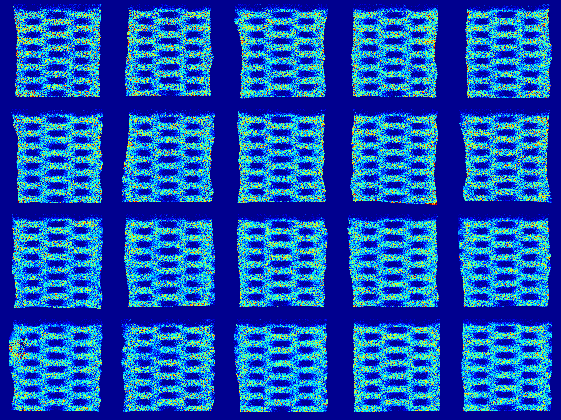
\includegraphics[width=3.6in]{figures/plan_data.png}

    \caption{The corrected flood data no longer presents dead pixels and hot spots.} \label{fig:UniCorr}
%\vspace{-0.2cm}
\end{figure}

The instability of the detectors leads to many repeat measurements which proved time-consuming. The need for a calibration procedure that can be quickly reproduced is essential to carry out the necessary corrections. We look to develop a calibration software that can account for new protocols. 
